%% joser_template.tex
%% V1
%% 2008/12/15
%% by Davide Brugali
%% This is a skeleton file demonstrating the use of joser1.cls
%% with a JOSER paper
%%
%% This file is a modified version of bare_jrnl_compsoc.tex V1.3
%% by Michael Shell for IEEE CS journal papers
%% http://www.michaelshell.org/
%%
%%*************************************************************************
%% Legal Notice:
%% This code is offered as-is without any warranty either expressed or
%% implied; without even the implied warranty of MERCHANTABILITY or
%% FITNESS FOR A PARTICULAR PURPOSE!
%% User assumes all risk.
%% In no event shall JOSER or any contributor to this code be liable for
%% any damages or losses, including, but not limited to, incidental,
%% consequential, or any other damages, resulting from the use or misuse
%% of any information contained here.
%%
%% This work is distributed under the LaTeX Project Public License (LPPL)
%% ( http://www.latex-project.org/ ) version 1.3, and may be freely used,
%% distributed and modified. A copy of the LPPL, version 1.3, is included
%% in the base LaTeX documentation of all distributions of LaTeX released
%% 2003/12/01 or later.
%% Retain all contribution notices and credits.
%% ** Modified files should be clearly indicated as such, including  **
%% ** renaming them and changing author support contact information. **
%%
%%*************************************************************************

% Fixes by Dave
\setlength{\paperheight}{11in}
\PassOptionsToPackage{pdfpagelabels=false}{hyperref} 



\documentclass[10pt,journal,compsoc]{joser1}

% *** GRAPHICS RELATED PACKAGES ***
%
\ifCLASSINFOpdf
   \usepackage[pdftex]{graphicx}
\else
   \usepackage[dvips]{graphicx}
\fi

%%%%%%%%%%%%%%%%%%%%%%%%%%%%%%%%%%%%%%%%%%%%%%%%%%%%%%%%%%%%%%%%%%%%%%%
%%%%%%%%%%%%%%%%%%%%%%% will be inserted by the editor %%%%%%%%%%%%%%%%
%%%%%%%%%%%%%%%%%%%%%%%%%%%%%%%%%%%%%%%%%%%%%%%%%%%%%%%%%%%%%%%%%%%%%%%
\journalnumber{1}                       %will be inserted by the editor
\journalvolume{1}                       %will be inserted by the editor
\journalmonth{September}                %will be inserted by the editor
\journalyear{2013}                      %will be inserted by the editor
\articlefirstpage{1}                  %will be inserted by the editor
\articlelastpage{10}                   %will be inserted by the editor
\setcounter{page}{1}                  %will be inserted by the editor
%%%%%%%%%%%%%%%%%%%%%%%%%%%%%%%%%%%%%%%%%%%%%%%%%%%%%%%%%%%%%%%%%%%%%%%

\copyrightauthor{D. Coleman, N. Correll}
\headoddname{F. A. AUTHOR et al./ Preparation of Papers for {\sl Journal of Software Engineering for Robotics}}%

% correct bad hyphenation here
\hyphenation{op-tical net-works semi-conduc-tor}


\begin{document}
% paper title
\title{Reducing the Barrier to Entry of \\\vskip 0.3\baselineskip Complex Robotic Software}

\author{
David COLEMAN$^{1}$
\qquad
Nikolaus CORRELL$^{1}$
%\qquad
%Third AUTHOR$^2$

%%%%%%%%%%%%%%%%%%%%%%%%%%%%%%%%%%%%%%%%%%%%%%%%%%%%%%%%%%%%%%%%%%%%%%%
%%%%%%%%%%%%%%%%%%%%%%% will be inserted by the editor %%%%%%%%%%%%%%%%
%%%%%%%%%%%%%%%%%%%%%%%%%%%%%%%%%%%%%%%%%%%%%%%%%%%%%%%%%%%%%%%%%%%%%%%
\thanks{{\bf Regular paper} -- Manuscript received April 19, 2009;
revised July 11, 2009.}
%%%%%%%%%%%%%%%%%%%%%%%%%%%%%%%%%%%%%%%%%%%%%%%%%%%%%%%%%%%%%%%%%%%%%%%


\IEEEcompsocitemizethanks{\IEEEcompsocthanksitem This work was
supported by xxxxxxxx (No.xxxxxxxx) (sponsor and financial support
acknowledgment goes here).\protect\\

\IEEEcompsocthanksitem Authors retain copyright to their papers
and grant JOSER unlimited rights to publish the paper
electronically and in hard copy. Use
of the article is permitted as long as the author(s) and the journal are properly
acknowledged.}

} % end author

\address{
$^1$ Department of Computer Science, University of Colorado at Boulder,
430 UCB, Boulder, Colorado 80309-0430\\
%$^2$ Department of Computing and Electronic Systems, University of
%Essex Colchester CO43SQ, UK 
}


% The paper headers
\markboth

\IEEEcompsoctitleabstractindextext{%
\begin{abstract}
Developing robot-agnostic software frameworks involves synthesizing many disparate fields of software engineering and robotic theory while at the same time accounting for a large variability in hardware designs and control paradigms. As the capabilities and power of robotic software frameworks increases, the complexity and learning curve to new users also increases. If the learning curve for applying and using the software on robots is too high, even the most powerful of frameworks is useless. A growing need exists in robotic software engineering to aid users in getting started with and customizing the provided components as necessary for particular robotic applications. In this paper a case study is presented for some of the best practices found for lowering the barrier of entry of the MoveIt motion planning framework that allows users to 1) quickly get basic motion planning functionality with very little initial setup, 2) automate the configuration and optimization of the framework where possible, 3) 
easily customize aspects of the tool-chain, and 4) benchmark the results of different configurations. A graphical interface that assists the user in configuring MoveIt is the cornerstone of our approach, together with a standardized robot model for input, automatically generated configuration files and launch files, as well as a plugin-based architecture for extensibility. These approaches for lowering the entry barrier are evaluated by a user survey and comparison against our design objects for their effectiveness to the users.

\end{abstract}

\begin{IEEEkeywords}
Robotic Software Frameworks, Motion Planning, Barrier to Entry, Setup, Usability, MoveIt
\end{IEEEkeywords}}



% make the title area
\maketitle


\section{Introduction}
% The very first letter is a 2 line initial drop letter followed
% by the rest of the first word in caps.
\IEEEPARstart{M}{anaging} {the increasing complexity of modern robotic software is a difficult engineering challenge faced by roboticists today. The size of the code bases of common open source robotic software frameworks such as ROS \cite{quigley2009ros}, MoveIt \cite{MoveIt} and OROCOS \cite{bruyninckx2001open} are swelling \cite{makarenko2007benefits}, and the required breadth of knowledge for understanding the deep stack of software from control drivers to high level planners is become more formidable. As it is beyond the capabilities for any one researcher to have the necessary domain knowledge for every aspect of a robot's tool chain, it is necessary to assist users in the configuration, customization, and optimization of the various software components of a robotic framework. 

\subsection{Barriers to Entry}

The term \textit{barriers to entry} is used here in the context of robotic software engineering to refer to the time, effort, and knowledge that a new user must invest in the integration of a software component to an arbitrary robot. This can include for example creating a virtual model of the robot's geometry and dynamics, customizing configuration files, choosing the fastest algorithmic approach for the application, and finding the best parameters for various algorithms. 

Powerful robotics software generally requires many varying degrees of customization and optimization for any particular robot to operate properly. Choosing the right parameters for each utilized algorithm and software component typically involves expert human input using domain-specific knowledge. Many new users to a software package, particularly as robotics becomes more mainstream, will not have the breadth of knowledge to customize every aspect of the tool chain. When the knowledge of a new user is insufficient for the requirements of the software, the barriers to entry become insurmountable and the software unusable. One of the emerging requirements of robot agnostic frameworks is implementing mechanisms that will automatically setup and tune the pipeline for arbitrary robots.

Another motivation for lowering the barrier to entry of complex robotics software is the \textit{paradox of the active user}. This paradox explains a common observation in many user studies that \textit{users never read manuals} but start attempting to use the software immediately \cite{carroll1987interfacing}. A user's desire to quickly accomplish a task results in them skipping reading any provided documentation or gaining deeper understanding of the system and instead diving right into completing their task. The \textit{paradox} is that the user would actually save time in the long run if they learned more about the system before attempting to use it, but from these studies it was that shown that in reality people do not tend to invest time upfront into learning a new system.

TODO: Paragraph on the need for quick start guides? Cite a paper on ''hello world'' type applications?

Even experts in the area of the associated robotics software will become frustrated if all initial attempts to setup and configure the framework fails and no progress is made. Researchers and engineers today do not have the time or ability to completely understand the entirety of robotics software before they start using it. It is very important for the first experience of the user with a piece of software be positive for the continued use of the software by the user.

\subsection{Benefits of Larger User Base}

The need to lower the barrier of entry is beneficial to the software itself in that it enables more users to utilize the framework. If the software framework is being sold for profit, the benefits of larger user base is obvious. If instead the software is a free open-source project, as most successful robotic frameworks currently are \cite{makarenko2007benefits}, lowering the barrier to entry is also beneficial in that it creates a larger community of users. As the number of users increases, the speed in which bugs are identified and fixed increases \cite{schmidt1999software}. It is also typically hoped that development contributions to the code base increases, though this correlation is not as strong \cite{schmidt1999software}. Additionally, one of the key strengths of a larger community for an open source project is increased participation of users assisting with quality assurance, documentation, and support \cite{schmidt2001leveraging}.

Another benefit of lowering the barrier of entry is it allows the robotics software to additionally become an educational tool for robotics. Not only is the software accessible for academic research and industrial applications, but undergraduate and even primary school students can use it learn some of the higher level concepts of robotic applications as has been demonstrated in \cite{correll2013one, moll2011teaching, }. This should not be the main focus of most robotics software, but a nice side effect.

\subsection{Related Work}

There has been much written and developed to addressed the software engineering challenges of complex robotic frameworks, but typically the identified design goals have emphasized the need for properties such as platform independence, scalability, real-time performance, software reuse, and distributed layouts \cite{realtime_framework, collett2005player, kramer2007development}. In \cite{kramer2007development}'s survey of nine open source robotic development environments, a collection of metrics were used which included documentation and graphical interfaces, but no mention was made of setup time, barrier to entry, or automated configuration. CITE MORE RELATED WORK

\subsection{Objectives}

In this paper we will be using the new MoveIt Motion Planning Framework as our case study for barriers of entry to the usage of robotics software. In section \ref{sec::motion_planning} we will discuss the many software components that make motion planning frameworks a good example of the difficulties of complex robotics software. In section \ref{sec::moveit} we will introduce the MoveIt motion planning framework, in section \ref{sec::lowering_barriers} the methods under taken in MoveIt to reduce the entry barriers will be discussed, and in section \ref{sec::results} we will present the results of these methods on the size of the user base and ease of adoption of the software framework. Will conclude with our experiences in the development process.

\section{Motion Planning Frameworks}
\label{sec::motion_planning}

Robotic motion planning is a maturing and central field in robotics \cite{moll2011teaching} that translates a task into a series of discrete motions such that a robot can move within its environment. The typical use case that will be used as an example in this paper is the problem of controlling a robotic arm from one configuration to another while taking into account various constraints.

The software development of a motion planning framework involves combining many disparate fields of robotics and software engineering \cite{perez2010roadmap}. We refer to the software as a \textit{framework} in this context because it abstracts the various components of motion planning into generic interfaces as discussed later.

One of the most important features of a framework for motion planning is providing the structures and classes to share common data between the different components. These basic data structures include a model of a robot with its collision bodies, a method for maintaining the state of the robot during planning and execution, and a method for maintaining the environment as perceived by the robot's sensors (''planning scene'').

In addition to the common data structures, a motion planning framework requires many different algorithmic components. The motion planning component itself includes one or more algorithms suited for the solving the expected planning problems a robot will encounter. The field of motion planning algorithms is large and no one-size fits all solution exists yet, so a framework that is robot agnostic should likely include an assortment of algorithms.

Other primary components include a collision checking module that detects the intersection of geometric primitives and meshes in the planning scene and robot model. A forward kinematics solver is required to propagate the robot's geometry based on its joint positions, and an inverse kinematics solver is required when planning in the configuration of an end effector. Other potential constraints, such as joint/velocity/torque limits, and stability requirements, require additional components.

Secondary components must also be integrated into a powerful motion planning framework. Depending on what configuration space a problem was solved in, a generated motion planning solution of position way points must be parameterized into a time-variant trajectory to be executed. A controller manager must decide the proper low level controllers for the necessary joints for each trajectory. Finally a perception interface must update the planning scene with recognized objects from a perception pipeline as well as optional raw sensor data.

Higher level applications are then built on top of these motion planning components to coordinate more complex tasks, such as pick and place routines. Other optional components of a motion planning framework can include benchmarking tools, introspection and debug tools, as well as user-facing graphical user interfaces. 

There already exists a number of motion planning frameworks available today, both open and closed source. A quick survey of these software projects... TODO SURVEY

\begin{itemize}
    \item ROS Arm Navigation
    \item OpenRave - Open Robotics Automation Virtual Environment
    \item OOPSMP - An Object-Oriented Programming System for Motion Planning
    \item MPK - Motion Planning Kit
    \item Motion Strategy Library
    \item Webots
    \item Custom software
\end{itemize}

\section{MoveIt Motion Planning Framework}
\label{sec::moveit}

MoveIt is the primary motion planning framework in ROS and has been successfully integrated with many robots including the PR2 \cite{wyrobek2008towards}, Robotnaut \cite{ambrose2000robonaut}, Baxter, and Atlas. It is written entirely in C++ but includes Python bindings for higher level scripting. It follows the principle of software reuse as advocated for robotics in \cite{makarenko2007benefits} of not tying itself exclusively to one robotic framework - in our case ROS - by creating a formal separation between core functionality and the framework-dependent aspects. 

By default the MoveIt Motion Planning Framework using the Open Motion Planning Library (OMPL) \cite{sucan2012the-open-motion-planning-library} for planning, the Fast Collision Library (FCL) \cite{fcl} for collision checking, and the OROCOS Kinematics and Dynamics Library (KDL) \cite{kdl} for forward and inverse kinematics. 

MoveIt is fast and can generate complete pick and place plans for a typical robotic arm in BENCHMARK TIME in preliminary experiments on an 64 bit Ubuntu 12.04 PC with a 3.6Ghz Intal Core i7 processor and 16 GB ram.

THINK OF MORE THINGS TO SAY

\section{Configuration Design Principles}
\label{sec::requirements}

In designing the configuration process required to allow MoveIt to work with many different types of robots using almost any combination of planning components, several contending design principles emerged. We believe these configuration design principles transcend motion planning and can be applied to most robotic software. 

{\bf Quick Start}: The amount of time required to accomplish the most primitive task expected from the robotic software component should be minimized. This is similiar to the time-honored ''Hello World'' demo frequently used by programming languages. This is essential for the \textif{paradox of the active user} as it provides cursory feedback to the user that the software works


\section{Methods to Lower The Entry Barrier}
\label{sec::lowering_barriers}

There are many challenges faced in created motion planning software that 


The following features have been implemented in MoveIt with the motivation to lower the barrier of entry for as many users as possible.

\subsection{Basic Motion Planning Out of the Box}

{\bf MoveIt Setup Assistant}: One of the unique features of MoveIt is the ratio of its power and features to the required setup time. A beginner to motion planning can with very little effort take a kinematic model of an arbitrary articulated rigid body robot and execute motion plans in a virtual environment. With a few extra steps of setting up the correct hardware interfaces, one can then execute the motion plans on their actual robotic hardware.

The main facility that provides out of the box support for beginners is the MoveIt Setup Assistant (SA). The SA is a graphical user interface that steps new users though the initial configuration requirements of using a custom robot with the motion planning framework (Figure 1). It accomplishes the task for the user of automatically generating many configuration files necessary for the initial operation of MoveIt. These configurations include a self-collision matrix, planning group definitions, robot poses, end effector semantics, virtual joints list, and passive joints list. A three dimensional model of the robot as its being configured is displayed on the right side of the SA graphical user interface (GUI) and various links on the robot are highlighted during configuration to visually confirm the actions of the user, as shown in Figure \ref{fig:setupassistant}.

\begin{figure}[!t]
\centering
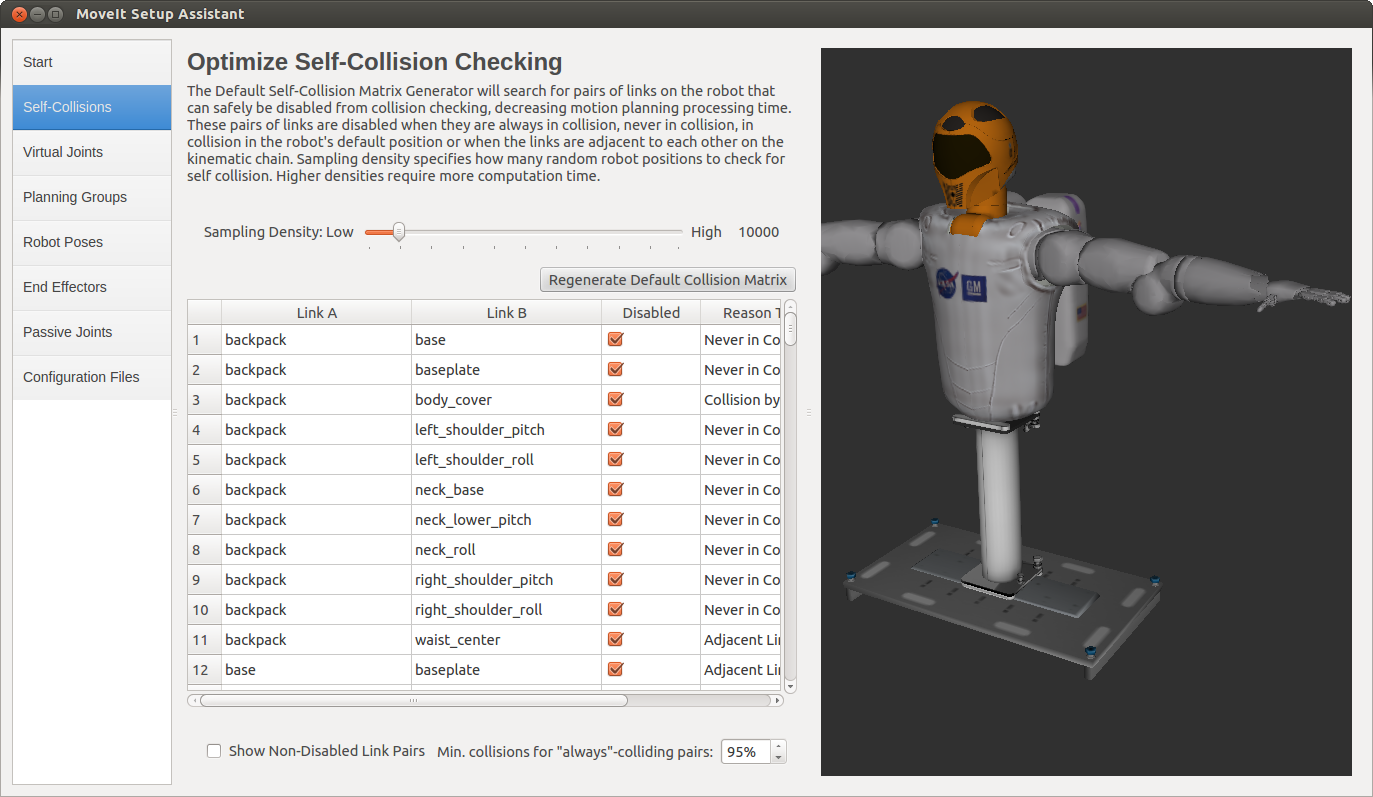
\includegraphics[width=3.4in]{images/setup_assistant}
\caption{Screenshot of MoveIt Setup Assistant with the Robonaut loaded TODO: better picture}
\label{fig:setupassistant}
\end{figure}

The required input for the SA is a robot model file, which currently accepts the Universal Robotic Description Format (URDF) \cite{garage2012xml} or Collada \cite{collada} file formats. These XML schemas describe the physical layout of a robot's link, joints, and other necessary modeling components. They can also combine appropriate 3D CAD meshes, collision models, dynamics, joint limits, sensors and other components. Using a properly formatted robot model file with the SA, MoveIt can automatically accomplish many of the required tasks in a motion planning framework including forward and inverse kinematics, collision checking, and joint limit enforcement.

If one truly desired, the steps within the SA could almost entirely be automated themselves, but they have been kept manual so as to allow edge cases and unusual customizations to be accomplished.

{\bf MoveIt Rviz Motion Planning Plugin}: The details of the automated configuration is left for the next section, but after the steps in the SA are completed the output is a ROS package containing a collection of configuration files and launch scripts. The launch files include a demo script that will startup a visualization tool (rviz) with the new robot loaded and ready to run state of the art motion planning algorithms in a non-physics based simulation. Using simple mouse-based interactive markers and the robot's various planning groups, the user can configure simple motion planning problems and quickly test the framework's capabilities.  

An example demo task would be using the mouse to drag a robot end effector from a start position to a goal position around some virtual obstacle. Using another GUI - the MoveIt Rviz Motion Planning Plugin - the user can click the \textit{Plan} button and observe MoveIt quickly plan the arm in a collision free path around the obstacle \ref{fig:motionrvizplugin}.

\begin{figure}[!t]
\centering
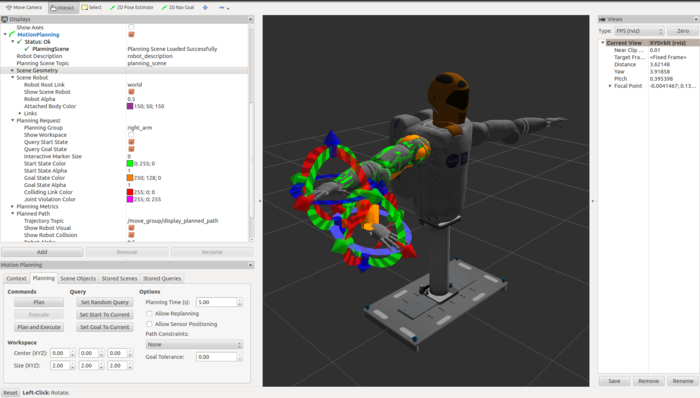
\includegraphics[width=3.4in]{images/rviz_plugin}
\caption{Screenshot of MoveIt Rviz Motion Planning Plugin with the Robonaut planning between two configurations TODO: better picture}
\label{fig:motionrvizplugin}
\end{figure}

It is important to emphasize the effect of a quick \textit{Getting Started} demo on a new user unaccustomed to MoveIt or motion planning in general. The reinforcement effect of initial success encourages the novice and enables them to start going deeper into the functionality and code base. If the entry barrier is too low, a new user will likely give up and turn to other frameworks or custom solutions rather than continue to blindly fix software that they have no experience in. TODO: move this paragraph?

{\bf Hardware Configuration and Execution}: Once the user is comfortable with the basic tools and features provided by MoveIt, the next step is to configure their robot's actual hardware actuators and control interfaces to accept trajectory commands from MoveIt. This step requires some custom coding to account for the specifics of the robot hardware - the communication bus, real-time requirements, and control theory implementations. At the abstract level, all MoveIt requires is that the robot hardware accepts a standard ROS trajectory message containing a discretized set of time-variant waypoints including desired positions, velocities, and accelerations. 

\subsection{Automate configuration and optimization}

The size and complexity of a feature-rich motion planning framework like MoveIt requires many parameters and configurations of the software be automatically setup and tuned. MoveIt accomplishes this both in the setup phase of a new robot - using the Setup Assistant - and sometimes during the runtime of the application.

{\bf Self Collision Matrix}: The second step of the SA is the generation of a self-collision matrix for the robot. This collision matrix encodes pairs of links on a robot that never need to be checked for self-collision due to the kinematic infeasibility of there actually being a collision. Reasons for having collision checking disabled between two links includes:
 
\begin{itemize}
    \item Links that can never reach each other kinematically
    \item Adjoining links that are connected and so are by design in collision
    \item Links that are always in collision for any other reason including inaccuracies in the robot model and precision error
\end{itemize}

This self-collision matrix is generated by running the robot through tens of thousands of random joint configurations and recording statistics of each link's collision status. The algorithm then automatically populates a list of link pairs that have been determined to never need to be collision checked. This saves future motion planning runs time because it reduces the amount of collision checks that are required.

{\bf Semantic Robotic Description Format}: The other six steps of the SA all provide graphical front ends for the data required to populate the semantic robotic description format (SRDF) file used by MoveIt. The SRDF provides meta data of the robot model useful to motion planning, such as which set of joints constitutes an arm and which set of links is considered part of the end effector. Requiring the user to configure all the required semantic information by hand in a text editor would be far more tedious and difficult than using an interface that populates the available options for each required field.

The last step of the SA is to generate all launch scripts and configuration files. Not only does this step involve outputting to file the collected configurations during the step-by-step user interface, but it all generates a series of default configuration and launch files that are customized for the particular robot using the URDF and SRDF information. These defaults include the velocity and acceleration limits for each joint, the kinematic solvers for each planning group, the available planning algorithms and projection evaluators for planning. Default planning adapters are setup for pre- and post-processing of motion plans, such as fixing slightly invalid start states and smoothing generated trajectories. Default benchmarking setups, controller and sensor manager scripts, and empty object databases are all generated. 

{\bf Internal Optimization}: TODO: I have emailed Ioan for his thoughts on this

\subsection{Easily customize aspects of the toolchain}

Out of the box MoveIt lowers the barrier to entry by not requiring the user to provide their own implementation of any of the components in the motion planning framework - the defaults are the aforementioned OMPL, FCL, and KDL software components. By default no perception components are configured

All these default choices however are limiting to more advanced users who have their own research or application-specific needs to fulfill. All of the just mentioned components are setup using plugin interfaces that are shared objects loaded at run time. Using common plugin interfaces, MoveIt can easily be customized by user created plugins for any or all of the motion planning components.

MoveIt is a plugin-centric framework that mostly avoids using message-passing inter-component communication, such as ROS messages. This decreases much of the latency delays inherent in message passing techniques and increases. The extensibility of the framework is greatly enhanced by not forcing users to use any particular algorithmic approach. Essentially, MoveIt provides a set of data sharing and synchronization tools, sharing between all components the robot's model and state.

One plugin in particular that MoveIt reduces the barrier to entry for customization is the inverse kinematics plugin. The default KDL plugin uses numerical techniques to convert from an end effector to joint configuration space. A must faster solution can be achieved by configuring OpenRave's IKFast \cite{ikfast} plugin that analytically solves the inverse kinematics problem. A combination of MoveIt scripts and the IKFast Robot Kinematics Compiler automatically generates the C++ code and plugin needed to increase the speed of motion planning solutions by up to 3 orders of magnitude.

TODO diagram of all possible plugin components in moveit

\subsection{Benchmark the results of different configurations}

The ability to configure and switch out motion planning algorithms and approaches is a powerful feature of MoveIt, but its usefulness is limited without the ability to quantify the results of any changes. Optimization criteria such as path length, planning time, smoothness, distance to nearest obstacle, and energy minimization need benchmarking tools to enable users and developers to find the correct set parameters and components for any given robotic application.

MoveIt again provides a low barrier to entry for benchmarking with easy to create benchmarking configuration files that allow each test to be setup for comparison against other algorithms and values. Multivariable parameter sweeps for finding the optimal value for an algorithm's performance can be accomplished by simply supplying a upper and lower search value as well as an increment amount. Results can be output into generic formats for use in different plotting tools.

TODO: expand this section. Cite Ben Cohen's paper on it

\section{Results}
\label{sec::results}

TODO 

Quantify MoveIt's popularity so far

Released 05/06/2013

Number of debian downloads? ask Tully to get this?

163 users on the MoveIt mailing list

Show plot of MoveIt posts over time

Show plot of users on mailing list over time

Show plots from https://www.ohloh.net/p/moveit

Survey on students and research's experience with MoveIt

\section{Remaining Issues}
\label{sec::issues}

TODO 

''Will conclude with our experiences in the development process.''

There are still barriers to entry

Setting up controllers is difficult

Large code base is intimidating

Built by one programmer so not the easiest layout

\section{Conclusion}

Beyond the usual considerations in building successful robotics software, an open source project that desires to maintain an active user base needs to take into account the barrier of entry to new users. As the algorithms become more complicated and the number of components and code base increases, configuring an arbitrary robot to utilize robotic software becomes a daunting task requiring domain-specific expertise in a very large breadth of theory and implementation. To account for this, quick and easy initial configuration, with partially automated optimization, and easily extensible components for future customization are becoming a greater necessity in motion planning and robotic software engineering in general. 

\section*{Acknowledgments}
The authors would like to thank...

% references section
\bibliographystyle{IEEEtran}
% argument is your BibTeX string definitions and bibliography database(s)
\bibliography{IEEEabrv,moveit_setup_bibliography}


% biography section
\begin{IEEEbiography}[{coleman}]{First Author}
received his B.\,Sc. and
M.\,Sc. degrees in mechanical engineering from the *** University,
in 1977 and 1984, respectively, and the Ph.\,D. degree in
computing from *** University, in 1992. In 1994, he was a
faculty member at *** University and in 1996 at ***
University. Currently, he is a professor in the Department of
Information System Engineering at *** University.
He has published about 100 refereed journal and conference papers.
His research interest covers robotics, software engineering, and distributed systems.
Prof. Author received research award from Science Foundation, and
the Best Paper Award of the XX International Conference in 2000 and
2006, respectively. He is a member of ACM and IEEE.
\end{IEEEbiography}

\begin{IEEEbiography}[{nikolauscorrell}]{Second Author}
received his B.\,Sc. and
M.\,Sc. degrees in mechanical engineering from the *** University,
in 1977 and 1984, respectively, and the Ph.\,D. degree in
computing from *** University, in 1992. In 1994, he was a
faculty member at *** University and in 1996 at ***
University. Currently, he is a professor in the Department of
Information System Engineering at *** University.
He has published about 100 refereed journal and conference papers.
His research interest covers robotics, software engineering, and distributed systems.
Prof. Author received research award from Science Foundation, and
the Best Paper Award of the XX International Conference in 2000 and
2006, respectively. He is a member of ACM and IEEE.
\end{IEEEbiography}


% insert where needed to balance the two columns on the last page with
% biographies

% You can push biographies down or up by placing
% a \vfill before or after them. The appropriate
% use of \vfill depends on what kind of text is
% on the last page and whether or not the columns
% are being equalized.

\vfill

% Can be used to pull up biographies so that the bottom of the last one
% is flush with the other column.
%\enlargethispage{-5in}

% that's all folks
\end{document}
